% ----------------------------------------------------------
% Protocolos de comunicaçào
% ----------------------------------------------------------
\chapter[Estudo de Caso]{Estudo de Caso}\label{cap:estudo}
%\addcontentsline{toc}{chapter}{Protocolos de Comunicação}
% ----------------------------------------------------------

Para obter um exemplo do mundo real, um estudo de caso foi projetado com base em uma aplicação de WMS (\textit{Warehouse Management System}). \citeonline{wms-definition} explica que um sistema de WMS é um software que auxilia as operações do dia-a-dia em um armazém. Os sistemas WMS permitem o gerenciamento centralizado de tarefas, como o rastreamento de níveis de inventário e locais de estoque. Tais sistemas WMS podem ser um aplicativo independente ou parte de um sistema de ERP.

Com o intuito de realizar consultas relevantes, foi modelado um esquema contendo seis entidades capazes de representar consultas reais, e ainda produzirem informações pertinentes para uma análise de desempenho. A construção das APIs seguiram os princípios do ciclo tradicional do desenvolvimento de \textit{software}, portanto a modelagem foi elaborada antes do início da implementação das APIs. Isso assegura que nenhuma decisão de tecnologia tenha afetado a modelagem das entidades.

A modelagem da figura \ref{fig:modelagem}, representa o gerenciamento de um armazém com capacidade de armazenar diversos itens. Os itens são dispostos em \textit{pallets}, e alocados em endereços dentro do armazém. Como pode ser observado na figura \ref{fig:rack}, os endereços do armazém são formados a partir de uma combinação de três dimensões: \textbf{Prateleira}, \textbf{Linha} e \textbf{Nível}. Cada combinação dessas três propriedades é capaz de alocar \textit{pallets}, que por sua vez podem conter diversas unidades de um mesmo item.

\begin{figure}[htbp]
\centering
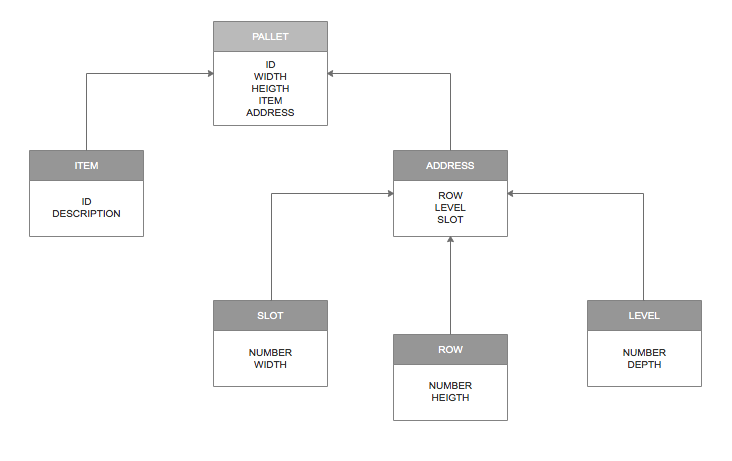
\includegraphics[width=0.9\textwidth]{figuras/model.png}
\caption{Modelagem WMS}
\label{fig:modelagem}
\end{figure}

Imagine um item de código 22B12, por exemplo, que representa um dado produto X. Este produto é disposto em um \textit{pallet} com capacidade de armazenar 30 unidades do item 22B12. O armazém é composto por 26 prateleiras, sequenciadas de 'A' a 'Z'. Cada prateleira possui 2 linhas de profundidade e 3 níveis de altura. Um \textit{pallet} com o código 001 contém 30 unidade do item 22B12, e precisa ser alocado dentro armazém, para isso é utilizado um sistema de códigos envolvendo as 3 dimensões do armazém.

\begin{figure}[htbp]
\centering
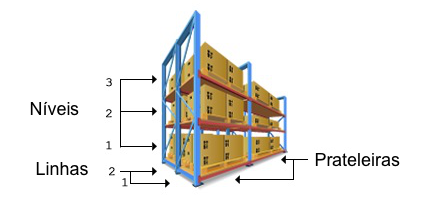
\includegraphics[width=0.7\textwidth]{figuras/rack.png}
\caption{Diagrama de dimensões do armazém}
\legend{Fonte: \citeonline{wms-rack}}
\label{fig:rack}
\end{figure}

Desta forma, 60 unidades do item 22B12 estão dispostos em dois \textit{pallets}(001, 002) existentes no armazém, e cada um dos \textit{pallets} será destinado a um endereço. O \textit{pallet} 001 será alocado na terceira prateleira, no segundo nível e na primeira linha. Após a formação do endereço, o \textit{pallet} 001 estará localizado no endereço C0201, prateleira C, nível 02 e linha 01.

Baseado em um sistema de WMS, dois protótipos de APIs serão implementados para uma análise. A primeira API será implementada seguindo as melhores práticas do \textit{design} do REST, descritas na sessão \ref{sec:rest}. A segunda será desenvolvida utilizando o GraphQL, e o seu desempenho será comparado com a API REST.

\section{Hipóteses} \label{sechHipóteses}

As hipóteses na diferença de desempenho entre as APIs derivaram dos fundamentos teóricos. Elas baseiam-se no entendimento de que os protocolos utilizados possibilitam a implementação de uma combinação de técnicas afim de afetar positivamento o desempenho da API. Portanto, ambas as implementações devem ter as mesmas propriedades, seguindo suas melhores práticas, modelos de maturidade e documentação.

As hipóteses deste trabalho são: 

\begin{enumerate}[label=\alph*)]
\item O tamanho da resposta será menor utilizando GraphQL;
\item O tempo de resposta será menor utilizando GraphQL;
\item O tempo de utilização da CPU será menor utilizando REST;
\item O consumo de memória será menor Utilizando REST;
\end{enumerate}

Com o propósito de validar as hipóteses definidas, foram determinadas duas perguntas que envolvessem todas as entidades. Para cada pergunta existe apenas uma resposta correta e sua lógica é baseada em campos das estruturas de dados de retorno.

\textbf{Questão 1}: Qual item ocupa a maior quantidade de \textit{pallets} alocados no armazém?

\textbf{Questão 2}: O item com o código 22B12 está armazenado em quais endereços?

Desta forma, buscas serão realizadas tanto na API REST quanto na API GraphQL afim de recuperar as informações necessárias para a formulação das respostas. Para realizar estas buscas, medir o desempenho das APIs processando suas respostas e compara-los, algumas ferramentas foram utilizadas durante este trabalho. Estas ferramentas estão descritas na sessão \ref{sec:ferramentas}.

\section{Ferramentas utilizadas} \label{sec:ferramentas}

A escolha das ferramentas a serem usadas na implementação foi uma das partes mais importantes no planejamento do estudo de caso. Foi necessário pensar em uma especificação que apresentasse uma curva rápida de aprendizagem, um fluxo de execução replicável e independente de plataforma, e uma documentação madura em relação à implementação das APIs.

As APIs foram escritas na linguagem de programação JavaScript, utilizando a especificação do ECMAScript 5. Foi escolhida esta linguagem devido ao fácil acesso a boas ferramentas para construção de serviços Web, como o Node.js. Node.js é uma plataforma para desenvolvimento de servidores Web utilizando JavaScript e o V8 JavaScript Engine. Assim, com Node.js pode-se criar uma variedade de aplicações Web utilizando código em JavaScript \cite{node-definition}.

\subsection{Ferramentas servidor}

Node.js dispõe de inúmeros recursos e ferramentas que possibilitam a construção de APIs. Mesmo assim, o ecosistema de bibliotecas no Node.js conta com ferramentas que simplificam ainda mais a construção de aplicações para servidores Web. Abaixo são citadas algumas bibliotecas que foram utilizadas para desenvolver tanto a API REST quando a API GraphQL. 

\subsubsection*{Express.js}

Express.js é um \textit{framework} para Node.js extremamente flexível, que fornece um conjunto robusto de ferramentas para a construção de aplicações Web e Móveis. Conta com um robusto sistema de roteamento, facilitando o desenvolvimento de APIs. O Express.js fornece uma fina camada de abstração nas principais funcionalidades do Node.js, sem sobrepor seus recursos.

Nos protótipos desenvolvidos para executar o experimento, o Express.js atua como um \textit{middleware}, gerenciando as rotas e delegando a responsabilidade de interpretação das requisições para os \textit{Controllers} na API REST e para os \textit{Resolvers} na API GraphQL.

O código \ref{lst:load-rest} ilustra como os \textit{Controllers} enviam as informações da requisição para o modelo, que é o responsável na API REST em executar as consultas no banco de dados. No exemplo abaixo, o trecho de código é o responsável por retornar um \textit{Item} baseado no \textup{id} recebido como parâmetro da requisição. É possível observar que na linha 2 o modelo da entidade \textit{Item} é importado para ser utilizado no \textit{Controller}, e na linha 8, o método \textup{get}, cujo a lógica está implementada dentro do modelo, é invocado passando como parâmetro o \textup{id}.

\begin{lstlisting}[escapeinside={(*}{*)}, numbers=left, caption={Controller para buscar um item}, label=lst:load-rest,language=JavaScript]
//item.controller.js
import Item from '../models/item.model';

/**
 * Load item and append to req.
 */
function load(req, res, next, id) {
  Item.get(id)
    .then((item) => {
      req.item = item;
      return next();
    })
    .finally(e => next(e));
}

\end{lstlisting}

Já o código \ref{lst:express-graph} mostra como o Express.js gerencia a requisição recebida via método GET, e delega a responsabilidade para o \textup{schema.js}, onde está contida a lógica para a interpretação dos parâmetros da requisição, e retorna um objeto JSON com a devida resposta.

\begin{lstlisting}[escapeinside={(*}{*)}, numbers=left, caption={Express gerenciando rotas para GraphQL}, label=lst:express-graph,language=JavaScript]
//server.js
import express from 'express';
let app = express();

import schema from './schema.js';

app.get('/', (req, res) => {
    graphql(schema, req.query.query)
    .then((result) => {
        res.send(result);
    });
});

\end{lstlisting}

\subsubsection*{MongoDB}

MongoDB é um banco de dados \textit{open source} que utilizada um modelo de dados orientado a objetos. Ele tem como característica conter todas as informações importantes em um único documento, possuir identificadores únicos universais (UUID), possibilitar a consulta de documentos através de métodos avançados de agrupamento e filtragem, também conhecido como \textit{MapReducers}. Ao invés de usar tabelas e linhas, como os bancos de dados relacionais, o MongoDB usa uma arquitetura baseada em coleções e documentos.


\subsubsection*{Ferramentas clientes}

Algumas ferramentas foram utilizadas para se comportaram como clientes das APIs construídas, e foram responsáveis por executar as consultas nas APIs. O foco deste trabalho não é em cima das aplicação clientes, entretanto é importante conhecê-las pois são elas que invocarão as consultas como também é através delas que algumas métricas serão extraídas. O software Postman será usado fundamentalmente para a execução das buscas nas APIs.

O Postman é uma cadeia completa de ferramentas para desenvolvedores de APIs. Ele é uma ferramenta elegante e flexível usada para construir softwares conectados via APIs, de forma rápida, fácil e precisa.

Ele funciona como uma emulador para execução de consultas em APIs. Com ele é possível executar buscas utilizando qualquer dos métodos do protocolo HTTP, possibilitando personalização tando do corpo quanto dos \textit{headers} das requisições, se preciso. Junto com a resposta da consulta, o Postman traz também informações extremamente relevantes, como tempo que a API levou para responder e o tamanho em bytes contido na resposta. Estas funcionalidades, aliadas com a opção de executar um número personalizável de iterações para cada requisição, será a base para avaliar o desempenho das APIs REST e GraphQL.

\subsection{Ambiente}

A configuração da máquina utilizada para o teste de desempenho local é descrita na Tabela \ref{tab:computers}. As APIs REST e GraphQL foram construídas para responder às requisições recebidas, retornando respostas no formato JSON, a fim de gerar um fator de medição de desempenho da execução dos testes. Para a execução do experimento, apenas os softwares necessários estavam ativos. Portanto, ao executar as buscas, o servidor REST ou GraphQL estará ativo, além do servidor de banco de dados MongoDB, e a aplicação cliente Postman.

\begin{table}[htbp]
    \centering
    \begin{tabular}{| l | l | l |}
        \hline
        \textbf{Item} & \textbf{Computador 1} \\ \hline
        Marca         & Apple                 \\ \hline
        Modelo        & Macbook Air 13"       \\ \hline
        Processador   & Intel Core i5 1.6 GHz \\ \hline
        Memória       & 4 GB 1600 MHz DDR3    \\ \hline
        Disco rígido  & 128 GB SSD            \\ \hline
        Sistema       & macOS Sierra 10.12.6  \\ \hline
    \end{tabular}
    \caption{Especificação da máquina utilizada} \label{tab:computers}
\end{table}

\subsection{Detalhes da implementação REST}

O servidor REST consiste em um servidor HTTP escrito em Node.js que recebe as requisições HTTP. Dependendo do método e URL da requisição, roteia-o para o \textit{controller} correspondente. O \textit{controller} faz a consulta na base de dados do MongoDB. Ao realizar o gerenciamento das rotas, o servidor realiza os devidos registros de latência. Após a consulta, a resposta desejada é enviada de volta para o cliente. Esse fluxo acontece em qualquer cenário, independente do número de requisições desejadas.

No presente trabalho, como o objetivo é apenas medir o desempenho de consultas utilizando REST, todas as requisições utilizarão o método HTTP GET. Para as medições da API REST, a aplicação cliente enviará, por exemplo, uma requisição para recuperar todos os itens cadastrados. Como pode ser observado da tabela \ref{tab:rest-url}, é necessário executar uma busca do tipo \textup{/item}, que será interpretada pelo servidor REST, identificando qual é a rota responsável por essa requisição. O servidor consultará a base de dados retornando uma resposta no formato JSON, com todos os itens cadastrados na API. Esse fluxo é ilustrado na figura \ref{fig:rest-uml}

\begin{table}[htbp]
    \centering
    \begin{tabular}{| l | l |}
        \hline
        \textbf{URI} & \textbf{Descrição} \\ \hline
        /item & Consulta lista de itens \\ \hline
        /item/:id & Consulta item pelo id \\ \hline
        /pallet & Consulta lista de pallets  \\ \hline
        /pallet/:id & Consulta pallet pelo id  \\ \hline
        /address & Consulta lista de endereços \\ \hline
        /address/:id & Consulta endereço pelo id \\ \hline
        /slot & Consulta lista de prateleiras \\ \hline
        /slot/:id & Consulta prateleira pelo id \\ \hline
        /row & Consulta lista de linhas \\ \hline
        /row/:id & Consulta linha pelo id \\ \hline
        /level & Consulta lista de nível \\ \hline
        /level/:id & Consulta nível pelo id \\ \hline
    \end{tabular}
    \caption{Servidor REST} \label{tab:rest-url}
\end{table}

\begin{figure}[htbp]
\centering
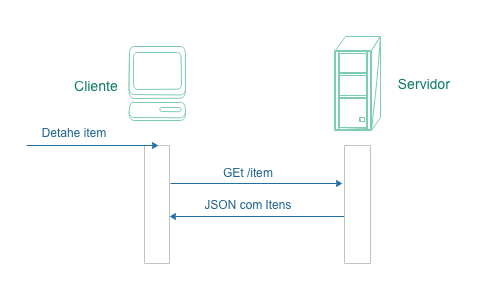
\includegraphics[width=0.8\textwidth]{figuras/uml-rest.png}
\caption{Fluxo REST}
\label{fig:rest-uml}
\author{fonte: Autor}
\end{figure}

\subsection{Detalhes da implementação GraphQL}

O servidor GraphQL foi implementado também usando Node.js. A diferença em comparação com a implementação do servidor REST é que o servidor GraphQL envia todos os pedidos ao seu núcleo, ao invés de rotear as requisições recebidas para vários \textit{controllers} diferentes. O GraphQL analisa a consulta e envia os parâmetros para os \textit{resolvers} responsáveis, localizados nos \textit{schemas}. \textit{Resolvers} são funções definidas para todos os campos no \textit{schema}, cada um retorna os dados para o campo específico. Estas funções são executadas quando os campos correspondentes são consultados e os resultados são retornados na resposta.

\begin{lstlisting}[escapeinside={(*}{*)}, numbers=left, caption=Consulta de itens, label=lst:query-graph, language=JavaScript]]
query RootQuery {
	items {
    	id
    	description
    }
}

\end{lstlisting}

 A consulta ilustrada do trecho de código \ref{lst:query-graph} solicita ao servidor GraphQL a lista a de todos os itens cadastrados na base de dados. Note no trecho de código \ref{lst:response-graph} que a resposta contém apenas os atributos que a consulta requisitou, ou seja, o \textup{id} e a descrição dos itens:

\begin{lstlisting}[escapeinside={(*}{*)}, numbers=left, caption=Listagem dos itens, label=lst:response-graph, language=JavaScript]]
{
    "data": [
         {
            "id": 22B12,
            "description": "Flat screen"
        },
        {
            "id": 21C44,
            "description": "Computer screen"
        },
        {
            "id": 43F12,
            "description": "Smartphone screen"
        },
    ]
}

\end{lstlisting}

Para recuperar alguma informação na API GraphQL, é necessária realizar uma requisição utilizando o método HTTP GET, passando como parâmetro a consulta desejada. A API irá então processar a consulta, e retornar um objeto JSON como a resposta da requisição. Detalhes deste fluxo estão ilustrados na figura \ref{fig:graph-uml}

\begin{figure}[htbp]
\centering
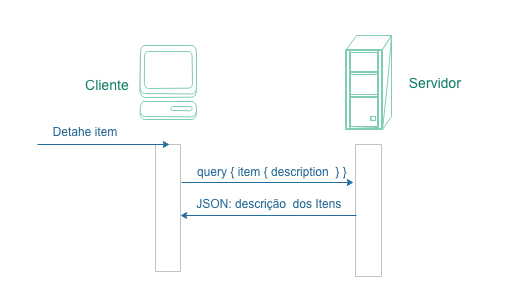
\includegraphics[width=0.8\textwidth]{figuras/uml-graph.png}
\caption{Fluxo GraphQL}
\label{fig:graph-uml}
\end{figure}

\section{Métricas}\label{sec:metrics}

A fim de comparar as medidas de desempenho de APIs desenvolvidas em REST com APIs desenvolvidas em GraphQL, algumas métricas precisam ser definidas. O desempenho de cada API vai depender de sua implementação, porém, escolhendo as métricas corretas, o efeito da implementação pode ser reduzido. Focando em medições corretas, as diferenças relevantes das APIs podem ser destacadas e melhor ponderadas.

Para o presente trabalho, serão utilizadas quatro métricas diferentes: O tempo de utilização da CPU, Consumo de memória, Tempo de resposta e o Tamanho da resposta. É importante ressaltar que cada métrica foi medida separadamente, para que \textit{logs} e \textit{outputs} pertinentes a uma métrica específica não interfira no resultado das demais.

\subsection*{Tempo de utilização da CPU}

O tempo de utilização da CPU é a quantidade de tempo para o qual uma unidade de processamento central (CPU) foi usada para processar instruções de um programa de computador ou sistema operacional

Esta métrica será extraída através do módulo \textit{process} presente no \textit{core} do Node.js. A função utilizada será a \textit{process.cpuUsage()} que trás como resultado o tempo gasto por um processo dentro da CPU, calculado pelo sistema operacional. A seguinte fórmula será usada para calcular esta métrica: 

$$ CPU = \frac{\sum\limits_{1}^{n} \Delta cpu}{n} $$

Onde $n$ é o número de CPUs e $\Delta cpu$ é o tempo de uso de CPU pela aplicação, sendo $\Delta cpu = T1 - T2$, em que $T1$ é o tempo final da execução e $T2$ é o tempo inicial. Nos resultados, esta métrica será apresentada na unidade de milissegundos (ms).

\subsection*{Consumo de memória}

O consumo de memória, junto com a utilização da CPU, é uma das medidas mais importantes pois são nesses pontos que observamos o verdadeiro custo computacional por trás da escolha da ferramenta. O consumo de memória é a quantidade de em bytes utilizada pela API, e será medido através da soma da utilização de memória em cada consulta necessária para atender os cenários propostos. A seguinte fórmula será usada para calcular esta métrica: 

$$ Mem = \frac{m}{M}*100 $$

Onde $m$ é a quantidade de memória usada pela aplicação e $M$ é o total de memória. Nos resultados, esta métrica será apresentada na unidade de megabytes.

\subsection*{Tempo de resposta}

É o tempo que cada requisição levou para realizar a consulta. Esse tempo é calculado a partir do início da requisição, até o retorno da resposta completa. No caso da API REST, esta métrica será cumulativa, ou seja, a soma do tempo de todas as requisições necessárias. A seguinte fórmula será usada para calcular esta métrica: 

$$ \Delta t = T1 - T2 $$

Onde $T1$ representa o tempo que a requisição respondeu a consulta, e $T2$ o tempo que foi solicitado a requisição. Nos resultados, esta métrica também será apresentada na unidade de milissegundos (ms).

\subsection*{Tamanho da resposta}

O tamanho da resposta será calculada baseado no tamanho em \textit{bytes} da resposta. Novamente, para a API REST será usada a média das somas de todas as consultas necessárias para obter a resposta desejada. A seguinte fórmula será usada para calcular esta métrica: 

$$ Tam = \sum\limits_{1}^{n} ti $$

Onde $ti$ é o tamanha da resposta de uma requisição, d $n$ é o número total de requisições. Nos resultados, esta métrica será apresentada na unidade de kilobytes.

A figura \ref{fig:my-metrics} mostra como as métricas serão extraídas. A utilização do CPU e o consumo de memória serão medidas utilizando ferramentas do próprio Node.js. Ambas serão medidas via \textit{logs} no código fonte dos protótipos implementados. O tamanho da resposta e o tempo de resposta serão extraídos utilizando a ferramenta Postman, ao final de cada consulta.

\begin{figure}[htbp]
\centering
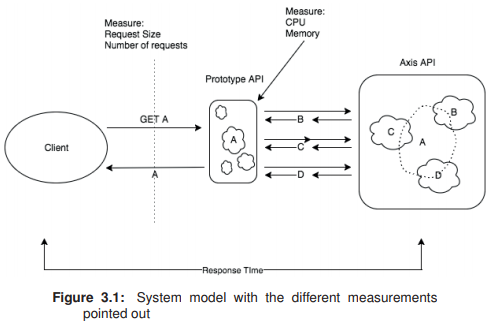
\includegraphics[width=0.8\textwidth]{figuras/metricas.png}
\caption{Arquitetura das APIs e diferentes pontos de medidas}
\label{fig:my-metrics}
\author{fonte: Autor}
\end{figure}

Afim de obter resultados mais precisos, serão feitas diversas iterações para medição de cada umas das métricas. A média destas medições será calculada através da segunte fórmula: 

$$ Avg = \frac{\sum\limits_{1}^{n} X}{n} $$

Onde $n$ é numero de iterações realizadas para cada métrica, e $X$ é o resultado de cada uma destas iterações.

Após a realização dos testes, os dados provenientes de cada uma das métricas foram coletados, analisados e os resultados serão apresentados no próximo capítulo. 